%========================= 参考文献 =========================
\bibliography{src/E-Reference}
\nocite{*}      % 引用所有的参考文献,不论是否被引用



%========================= 附录 =========================

\appendix
\section{程序代码}

\begin{lstlisting}[caption={搜索代码}]
import java.util.*;

public class Main {
    public static void main(String[] args) {
        Scanner input = new Scanner( System.in);

        double d0509, d0809, d0508;
        d0509 = input.nextDouble();
        d0809 = input.nextDouble();
        d0508 = input.nextDouble();


        double x = Math.sqrt(d0509*d0509 - ((d0509*d0509 - d0508*d0508 - d0809*d0809)/(2*d0809)));
        double y = (d0509*d0509 - d0508*d0508)/(2*d0809);
        

        System.out.println("x = "+x);
        System.out.println("y = "+y);
    }
}
\end{lstlisting}


\section{三圆定点模型示意图}

\begin{figure}[h]
    \centering
    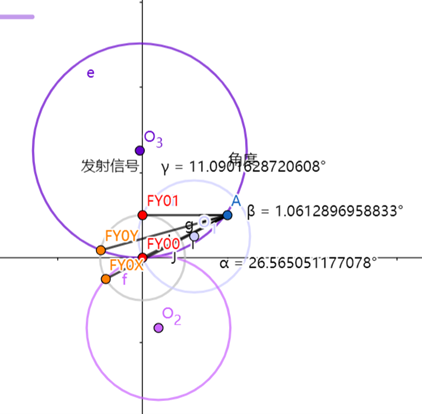
\includegraphics[scale=0.7]{res/figure111148.png}
    \caption{示意图一}
\end{figure}

\begin{figure}[h]
    \centering
    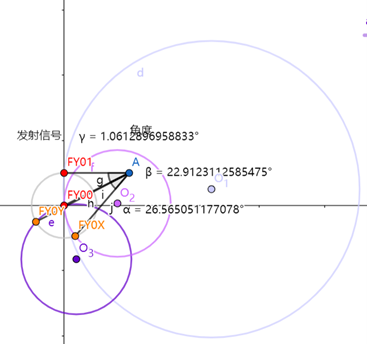
\includegraphics[scale=0.7]{res/figure111149.png}
    \caption{示意图二}
\end{figure}

